
\documentclass[tikz,border=12pt]{standalone}
\usepackage{pgfplots}
\pgfplotsset{compat=1.18}
\usetikzlibrary{arrows.meta,positioning,fit,calc}
\definecolor{ink}{HTML}{172026}
\definecolor{muted}{HTML}{5F6B73}
\definecolor{line}{HTML}{CBD5E1}
\definecolor{panel}{HTML}{F8FAFC}
\definecolor{bfs}{HTML}{64748B}
\definecolor{spine}{HTML}{0F766E}
\definecolor{hrg}{HTML}{7C3AED}
\definecolor{warn}{HTML}{C2410C}
\definecolor{ok}{HTML}{15803D}
\definecolor{blue}{HTML}{2563EB}
\pgfplotsset{
  every axis/.append style={
    tick label style={font=\small, color=ink},
    label style={font=\small, color=ink},
    title style={font=\bfseries\small, color=ink},
    legend style={font=\footnotesize, draw=none, fill=none},
    grid=major,
    grid style={line!55},
    axis line style={line},
  }
}
\begin{document}

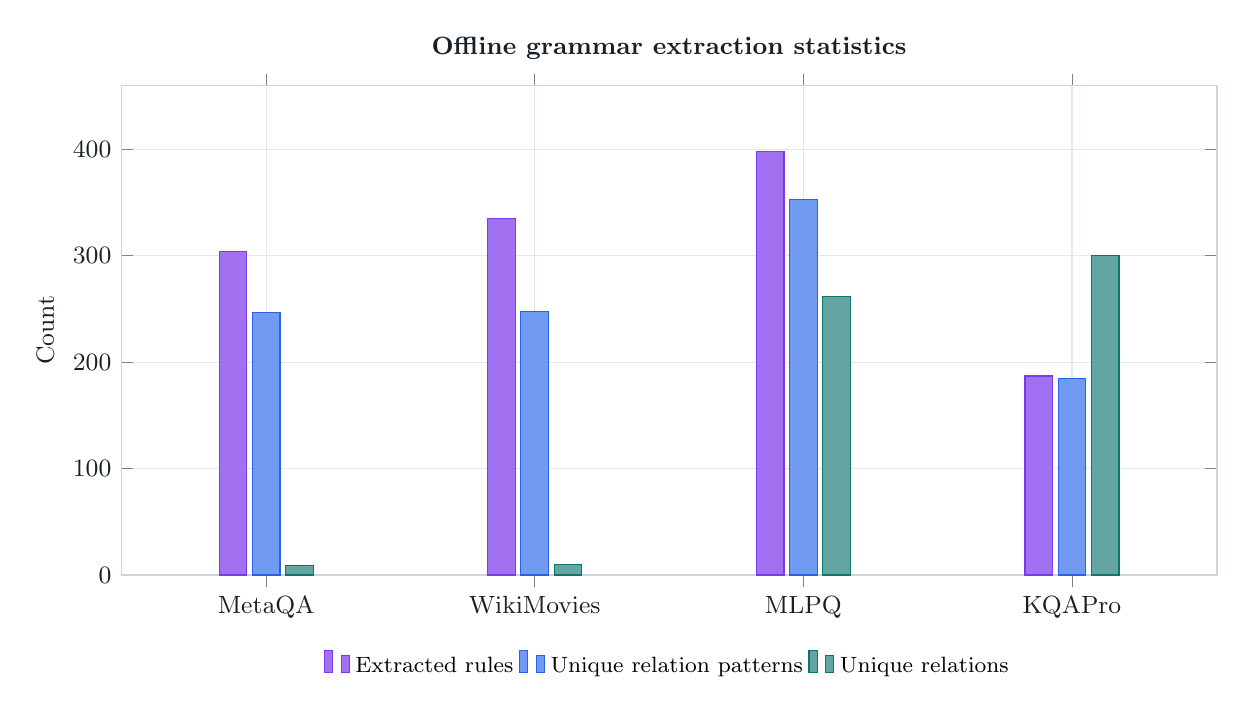
\begin{tikzpicture}
\begin{axis}[
  ybar,
  bar width=10pt,
  width=15.5cm,
  height=7.8cm,
  ymin=0,
  ymax=460,
  enlarge x limits=0.18,
  ylabel={Count},
  symbolic x coords={MetaQA,WikiMovies,MLPQ,KQAPro},
  xtick=data,
  x tick label style={rotate=0, font=\small},
  legend columns=3,
  legend style={at={(0.5,-0.14)}, anchor=north, font=\footnotesize},
  title={Offline grammar extraction statistics},
]
\addplot+[fill=hrg!72, draw=hrg] coordinates {(MetaQA,304) (WikiMovies,335) (MLPQ,398) (KQAPro,187)};
\addplot+[fill=blue!65, draw=blue] coordinates {(MetaQA,247) (WikiMovies,248) (MLPQ,353) (KQAPro,185)};
\addplot+[fill=spine!65, draw=spine] coordinates {(MetaQA,9) (WikiMovies,10) (MLPQ,262) (KQAPro,300)};
\legend{Extracted rules, Unique relation patterns, Unique relations}
\end{axis}
\end{tikzpicture}

\end{document}
